\chapter{Specific Details on Training Activities and Report}
\label{chapter-3}

\section{Introduction}
\begin{itemize}
    \item \textbf{Duration:} October 13, 2025 to December 5, 2025 (8 weeks)
    \item \textbf{Host Organization:} Tanbel Inc. (Parent of WeCycle and ArrayQ)
    \item \textbf{Key Focus Areas:} Full-Stack Web Development, Mobile App Maintenance, Payment Systems
    \item \textbf{Technologies Used:} React.js, Next.js, TypeScript, Capacitor, Stripe, Docker, Jira
    \item \textbf{Professional Growth:} Enhanced problem-solving skills, learned agile workflows, improved code quality practices
\end{itemize}

\section{Weekly Duties and Activities}

\section{Weekly Duties and Activities}

\subsection{Week 1: Bootstrapping \& Environment Setup (October 13-17, 2025)}
\begin{itemize}
    \item \textbf{WCAPP-1:} Explored the Capacitor dev workflow and set up the mobile app development environment.
    \item \textbf{WCAPP-3:} Optimized project structure and dependencies to reduce CI/CD build times.
    \item \textbf{WCAPP-38:} Fixed navigation persistence issues in the mobile app.
    \item \textbf{WCAPP-39:} Resolved safe area view issues on mobile devices.
    \item \textbf{WCAPP-56:} Added splash screen and app logo resources.
    \item \textbf{WCAPP-86:} Fixed user time zone mismatches for booking times.
\end{itemize}
\textbf{Key Learning:} Setting up a complex mobile/web hybrid environment (Capacitor), understanding CI/CD pipelines, and debugging mobile-specific UI issues.

\subsection{Week 2: Infrastructure \& Deployment (October 20-24, 2025)}
\begin{itemize}
    \item \textbf{WCAPP-85:} Synced staging database with production for accurate testing.
    \item \textbf{WCAPP-89:} Provisioned a DigitalOcean Droplet and configured Docker/Node.js services.
    \item \textbf{WCAPP-90:} Deployed the new Chatbot service, setting up SSL and domains.
    \item \textbf{WCAPP-36:} Integrated AI chat features into the staging environment.
    \item \textbf{WCAPP-23:} Adjusted booking start times to align with backend slots.
    \item \textbf{WCAPP-96:} Hotfixed invoice creation errors for existing bookings.
    \item \textbf{WCAPP-99/113:} Fixed web server errors and cache revalidation for dynamic content.
\end{itemize}
\textbf{Key Learning:} DevOps basics (Docker, DigitalOcean), Chatbot integration, and handling server-side caching strategies.

\subsection{Week 3: Data Management \& Optimization (October 27-31, 2025)}
\begin{itemize}
    \item \textbf{WCAPP-120:} Implemented CSV export for junk removal items and pricing.
    \item \textbf{WCAPP-118/119:} Improved date formatting and fixed invoice provider names.
    \item \textbf{WCAPP-87:} Enhanced Hauler details page with contact info.
    \item \textbf{WCAPP-126:} Deployed production Chatbot instance.
    \item \textbf{WCAPP-136:} Initialized the new ArrayQ site project structure.
    \item \textbf{WCAPP-122:} Added "Delete Account" functionality for GDPR compliance.
\end{itemize}
\textbf{Key Learning:} Data export features, starting new projects (ArrayQ), and implementing sensitive account actions (deletion).

\subsection{Week 4: Branding \& ArrayQ Development (November 03-07, 2025)}
\begin{itemize}
    \item \textbf{WCAPP-103:} Added WeCycle logo to invoices and dynamic email/phone details.
    \item \textbf{WCAPP-141/142:} Set global theme colors and hauler states for ArrayQ.
    \item \textbf{WCAPP-138:} Migrated dashboard to ArrayQ domain with updated branding.
    \item \textbf{WCAPP-144:} Implemented dynamic logo switching on invoices based on the booking source.
    \item \textbf{WCAPP-143:} Fixed timezone-related failures in custom booking creation.
    \item \textbf{WCAPP-149:} Created Privacy Policy page for ArrayQ.
\end{itemize}
\textbf{Key Learning:} Multi-tenant branding strategies, handling different domains/themes in a single codebase, and timezone logic.

\subsection{Week 5: Deployment \& Role Management (November 10-14, 2025)}
\begin{itemize}
    \item \textbf{WCAPP-139/151:} Deployed ArrayQ site to production and staging.
    \item \textbf{WCAPP-152:} Configured BLOG\_MANAGER role access across domains.
    \item \textbf{WCAPP-153:} Updated mobile app assets for the new brand identity.
    \item \textbf{WCAPP-158:} Fixed author designation mismatches on the blog.
    \item \textbf{WCAPP-163:} Debugged discount calculation mismatches on staging.
    \item \textbf{WCAPP-79:} Implemented job completion flow directly from the dashboard.
    \item \textbf{WCAPP-40/174:} Prepared production mobile build and created support pages.
\end{itemize}
\textbf{Key Learning:} Role-Based Access Control (RBAC), App Store deployment preparation, and debugging financial logic (discounts).

\subsection{Week 6: UX Refinements \& Performance (November 17-21, 2025)}
\begin{itemize}
    \item \textbf{WCAPP-173:} Updated email triggers to request Trustpilot reviews.
    \item \textbf{WCAPP-178:} Investigated caching issues with the new blog layout.
    \item \textbf{WCAPP-184:} Resolved App Store review rejections.
    \item \textbf{WCAPP-185:} Redirected haulers to the specific ArrayQ dashboard.
    \item \textbf{WCAPP-172:} Fixed Table of Contents and image loading on blogs.
    \item \textbf{WCAPP-127/98:} Refactored Booking and Invoice IDs to be human-readable.
    \item \textbf{WCAPP-189:} Simplified UI to hide individual item prices (subtotal only).
\end{itemize}
\textbf{Key Learning:} optimizing user communication flows (emails, reviews), handling App Store compliance, and UX simplification.

\subsection{Week 7: Pricing \& Pre-Production (November 24-28, 2025)}
\begin{itemize}
    \item \textbf{WCAPP-192:} Updated specific item pricing on production.
    \item \textbf{WCAPP-140:} Implemented mandatory OTP phone verification.
    \item \textbf{WCAPP-193:} Set up a dedicated Pre-Production environment.
    \item \textbf{WCAPP-200/201:} Fixed discount fallback text and mobile pricing display.
    \item \textbf{WCAPP-159:} Updated ArrayQ mobile app ID for store compliance.
    \item \textbf{WCAPP-2/4:} Fixed SMTP configurations and invoice payment link generation.
\end{itemize}
\textbf{Key Learning:} Security implementation (OTP), environment management (Pre-Prod), and payment infrastructure (SMTP/Invoices).

\subsection{Week 8: Fintech \& Final Polish (December 01-05, 2025)}
\begin{itemize}
    \item \textbf{WCAPP-5:} Implemented Stripe Connected Accounts for Haulers.
    \item \textbf{WCAPP-6:} Fixed bugs in the existing invoice editing feature.
    \item \textbf{WCAPP-22/24:} Upgraded Next.js, React, and Nx versions; fixed build errors.
    \item \textbf{WCAPP-33:} Updated internal text configurations.
    \item \textbf{Documentation:} Finalized documentation and testing for handover.
\end{itemize}
\textbf{Key Learning:} Integrating complex payment gateways (Stripe Connect), maintaining dependency health (major version upgrades), and project handover.

\section{Key Projects}

\subsection{Project 1: ArrayQ Platform Development}
\begin{itemize}
    \item \textbf{Scope:} Launching the ArrayQ brand with a dedicated web landing page and mobile application features.
    \item \textbf{Objective:} Create a distinct identity for the dumpster rental service while maintaining backend integration with WeCycle.
    \item \textbf{Key Tasks:}
    \begin{itemize}
        \item Developed the ArrayQ landing page with SEO optimization and privacy policies.
        \item Implemented multi-tenant logic to switch themes/branding based on the domain.
        \item Updated the mobile app with ArrayQ splash screens, logos, and build IDs.
        \item Set up separate staging and production environments for ArrayQ.
    \end{itemize}
    \item \textbf{Tools Used:} Next.js, Tailwind CSS, Capacitor, DigitalOcean
    \item \textbf{Outcome:} Successfully launched ArrayQ on web and mobile stores with distinct branding.
    \item \textbf{My Role:} Lead developer for frontend branding and mobile configurations.
\end{itemize}

\subsection{Project 2: Invoice \& Payment System Modernization}
\begin{itemize}
    \item \textbf{Scope:} Overhauling the financial processing system for haulers and customers.
    \item \textbf{Objective:} Enable automated payouts, dynamic invoicing, and secure payment links.
    \item \textbf{Key Tasks:}
    \begin{itemize}
        \item Integrated Stripe Connected Accounts for direct hauler payouts.
        \item Refactored invoice generation to include dynamic logos and contact info.
        \item Fixed critical bugs in invoice editing and existing booking calculations.
        \item Implemented logic to hide item-specific pricing on mobile views for better UX.
    \end{itemize}
    \item \textbf{Tools Used:} Stripe API, React.js, Node.js (Backend logic understanding)
    \item \textbf{Outcome:} Streamlined the payment flow, reducing manual errors and support tickets.
    \item \textbf{My Role:} Full-stack implementation of payment features and invoice UI.
\end{itemize}

\subsection{Project 3: Chatbot \& Support Integration}
\begin{itemize}
    \item \textbf{Scope:} Deploying an AI-powered support assistant.
    \item \textbf{Features Implemented:}
    \begin{itemize}
        \item Deployed the Chatbot service on a custom DigitalOcean droplet.
        \item Configured SSL certificates and domain mapping.
        \item Integrated the chat widget into the production and staging sites.
    \end{itemize}
    \item \textbf{Tools Used:} Docker, Nginx, SSL/TLS, AI Chat SDKs
    \item \textbf{Outcome:} Reduced support team load by automating initial customer queries.
    \item \textbf{My Role:} DevOps configuration and frontend integration.
\end{itemize}

\section{Other Responsibilities}
\begin{itemize}
    \item \textbf{Code Reviews:} Participated in code review sessions, ensuring type safety and code quality.
    \item \textbf{Sprint Planning:} Attended sprint planning meetings to estimate story points for features.
    \item \textbf{Bug Reporting:} Documented reproduction steps for QA bugs in Jira.
    \item \textbf{Version Control:} Managed branching strategies and resolved release conflicts.
\end{itemize}

\section{Internship Summary}

\par This internship served as the definitive test of my academic training. While the B.Sc. curriculum provided the theoretical scaffolding, Tanbel Inc. introduced the volatility of a live production environment. The objective was clear: translate textbook concepts into shipping code. My role was comprehensive—spanning frontend, backend, and infrastructure—ensuring stability in a product used by real customers.

\par The remote nature of the work changed how I learned. No office meant no one over my shoulder. Results were the only thing that mattered. Jira wasn't just a tool; it was the entire workflow. I had to learn to navigate the codebase alone. I couldn't just raise my hand. I had to dig through docs and wait for Slack replies. It forced me to solve problems that textbooks don't cover.

\begin{figure}[H]
    \centering
    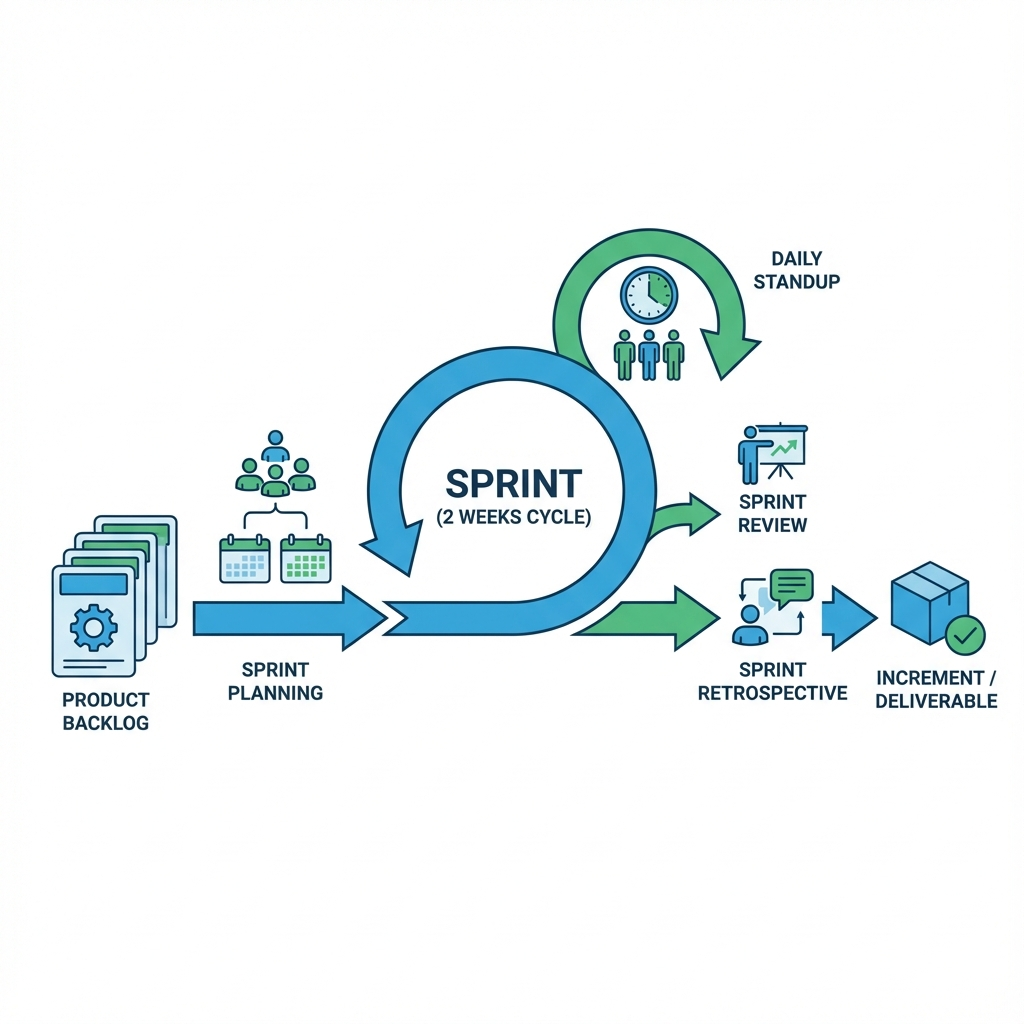
\includegraphics[width=0.85\textwidth]{figures/agile_workflow.png}
    \caption{Agile Scrum Workflow Used During Industrial Training}
    \label{fig:agile-workflow}
\end{figure}

\begin{table}[H]
\centering
\caption{Internship Summary}
\label{tab:internship-summary}
\renewcommand{\arraystretch}{1.4}
\begin{tabularx}{\textwidth}{|>{\centering\arraybackslash}p{5cm}|>{\arraybackslash}X|}
\hline
\textbf{Parameter} & \textbf{Details} \\
\hline
\textbf{Organization Name} & Tanbel Inc. (WeCycle \@ ArrayQ) \\
\hline
\textbf{Internship Period} & October 13, 2025 to December 5, 2025 \\
\hline
\textbf{Total Duration} & 8 weeks (40 working days) \\
\hline
\textbf{Total Working Hours} & 320 hours (40 hours/week) \\
\hline
\textbf{Mode of Internship} & Remote \\
\hline
\textbf{Nature of Work} & Full-Stack Engineering, Mobile App Maintenance, DevOps \\
\hline
\textbf{Tools and Technologies Used} & React.js, Next.js, TypeScript, Capacitor, Stripe, Docker \\
\hline
\textbf{Learning Methodology} & Task-based learning, Code reviews, Sprint cycles, Team collaboration \\
\hline
\textbf{Reporting Mechanism} & Jira (71 Issues Resolved), Daily Standups, Weekly Syncs \\
\hline
\textbf{Industrial Supervisor} & MD Tanvir Ahmed \\
\hline
\end{tabularx}
\end{table}

\par This bridge between theory and reality was necessary. Algorithms in class are neat; production code is messy. I didn't just get better at React. I learned how to build software that doesn't break when people use it. That shift—from student mindset to engineer mindset—is the most important part.